\documentclass{beamer}

\usepackage[utf8]{inputenc}
\usepackage[russian]{babel}
\usepackage{graphicx}
\usepackage{caption}
\usepackage{subcaption}

\usetheme{Madrid}


\title[ВКР]
{Гамильтонов формализм для задачи гарантированного синтеза управлений при геометрической неопределенности}

\author[Е. В. Гуров]
{студент 4 курса Е. В. Гуров \\
научный руководитель --- академик, д.ф.-м.н., проф.  \\ А. Б. Куржанский}

\institute[СА]
{ Кафедра системного анализа \\
факультета ВМК МГУ имени М.В. Ломоносова}

\date[31 мая 2022 г.]

\begin{document}

\frame{\titlepage}

\begin{frame}{Постановка задачи}
\footnotesize
Рассматривается система
\begin{equation*}
    \dot{x} = A(t)x + B(t)u + C(t)v(t)
\end{equation*}
Здесь:
\begin{itemize}
    \item \( x \in \mathbb{R}^n \) --- вектор состояния системы
    \item \( u \in \mathbb{R}^p \) --- управление
    \item \( v \in \mathbb{R}^q \) --- некоторое неизвестное внешнее возмущение
\end{itemize}
Известны "геометрические" \ ограничения на помеху и управление
\begin{equation*}
    v(t) \in \mathcal{Q}(t), \quad u(t) \in \mathcal{P}(t),
\end{equation*}
а также задано компактное целевое множество \( \mathcal{M} \in \text{comp} \, \mathbb{R}^n \). \\
Необходимо отыскать множество разрешимости \( \mathcal{W}(\tau, t_1, \mathcal{M}) = \mathcal{W}[\tau] \) и позиционное управление \( u = \mathcal{U}(t,x) \) такие, что все решения дифференциального включения
 \begin{equation*}\label{dif_inclusion}
    \dot{x} \in A(t)x + B(t)\mathcal{U}(t,x) + C(t)v(t), \quad t_0 \le t \le t_1, 
\end{equation*}
выпущенные из любой начальной позиции \( \{\tau, x_{\tau}\}, \, x_{\tau} = x(\tau), \, x_{\tau} \in \mathcal{W}(\tau, t_1, \mathcal{M}) \), \( \tau \in [t_0, t_1) \), достигали бы целевого множества \( \mathcal{M} \) в момент времени \( t_1 \) при любом внешнем неизвестном возмущени \( v(t) \in \mathcal{Q}(t) \).

\end{frame}


\begin{frame}{Редукция системы}
Приведем вначале систему к более простому виду
\begin{equation*}
    \dot{x} = u + v
\end{equation*}
с новыми ограничениями
\begin{equation*}
    u \in \mathcal{P}_0(t), \quad v \in \mathcal{Q}_0(t),
\end{equation*}
где \( \mathcal{P}_0(t) = G(t_1, t) B(t) \mathcal{P}(t), \, \mathcal{Q}_0 = G(t_1,t)C(t)\mathcal{Q}(t) \) и \( G(t_1,t) \) --- фундаментальная матрица однородного уравнения. Для этого сделаем замену \( x(t) = G(t_1, t)x(t) \).
\end{frame}

\begin{frame}{Уравнение Гамильтона-Якоби-Беллмана}
Введем функцию цены
\begin{equation*}
    \mathcal{V} = \min_{\mathcal{U}} \max_{x(\cdot)} \{\mathcal{I}(t,x) \mid \mathcal{U} \in 
     U_{\mathcal{P}}, \, x(\cdot) \in \mathcal{X}_{\mathcal{U}}(\cdot) \},
\end{equation*}
где
\[
     \mathcal{I}(t,x) = d^2(x[t_1], \mathcal{M})
\]
и \( \mathcal{X}_{\mathcal{U}}(\cdot) \) --- множество всех траекторий \( x(\cdot) \) включения
\begin{equation*}
    \dot{x} \in \mathcal{U}(t,x) + \mathcal{Q}(t), \quad x(\tau) = x,
\end{equation*}
порожденных заданной стратегией \( \mathcal{U} \).

В таком случае для функции \( \mathcal{V}(t,x) \) можно составить следующее уравнение 
 Гамильтона-Якоби-Беллмана-Айзекса:
\begin{equation*}
    \frac{\partial \mathcal{V}}{\partial t} + \min_u \max_v \left( \frac{\partial \mathcal{V}}
     {\partial x}, u + v \right) = 0, \quad u \in \mathcal{P}(t), \ v \in \mathcal{Q}(t),
\end{equation*}
с граничным условием
\begin{equation*}
    \mathcal{V}(t_1, x) = d^2(x, \mathcal{M}).
\end{equation*}

\end{frame}

\begin{frame}{Вид функции цены}
\small
Рассматриваемая задача с неопределенностью приводит к понятию альтернированного интеграла Понтрягина \( \mathcal{I}(t, t_1, \mathcal{M}) \).

\begin{block}{Теорема}
    Множество разрешимости \( \mathcal{W}[t] \) может быть представлено как 
    \begin{equation*}
        \mathcal{W}[t] \equiv \mathcal{I}(t, t_1, \mathcal{M}), \quad t_0 \le t \le t_1.
    \end{equation*}
\end{block}

С помощью альтернированного интеграла возможно получить явный вид для функции цены в данной задаче.

\begin{block}{Теорема}
Функция цены представляется в виде
    \begin{equation*}
        \mathcal{V}(\tau, x) = d^2(x, \mathcal{I}[t]) = d^2(x, \mathcal{W}[t]).
    \end{equation*}
\end{block}

Эта теорема даёт подход к построению управлений. Получается, что для минимизации функции цены необходимо строить управление, минимизирующее расстояние до множества разрешимости.

\end{frame}

\begin{frame}{Выражение для управлений}


Вернемся к уравнению Гамильтона-Якоби-Беллмана-Айзекса:
\[
        \frac{\partial \mathcal{V}}{\partial t} + \min_u \max_v \left( \frac{\partial \mathcal{V}}
         {\partial x}, u + v \right) = 0
\]

Если решение уравнения удается найти, то гарантирующая стратегия управления находится следующим образом:
\begin{equation*}
    \mathcal{U}_*(t,x) = \mathrm{argmin} \left\{ \left( \frac{\partial \mathcal{V}}{\partial x},
     u \right) : u \in \mathcal{P}(t) \right\},
\end{equation*}
если градиент \( \partial \mathcal{V} / \partial x \) существует в точке \( (t, x) \). Или в общем случае
\begin{equation*}
    \mathcal{U}_*(t,x) = \left\{ u: \max_v \{ dh_+^2(x, \mathcal{W}[t]) / dt : v \in \mathcal{Q}(t) \} 
     \le 0 \right\}.
\end{equation*}
    
\end{frame}

\begin{frame}{Система с эллипсоидальными ограничениями}
\footnotesize
Будем рассматривать систему
\begin{equation*}
    \dot{x} = u + v
\end{equation*}
с эллипсоидальными ограничениями
\begin{equation*}
    u \in \mathcal{E}(p(t), P(t)), \quad v \in \mathcal{E}(q(t), Q(t)), \quad \mathcal{M} = 
     \mathcal{E}(m, M).
\end{equation*}
Здесь функции \( p(t), q(t), P(t), Q(t) \) предполагаются заданными и непрерывными. Вектор \( m \) и
 матрица \( M \) фиксированы. Эллипсоиды задаются своим центром и матрицей следующим образом:
 
\begin{equation*}
    \mathcal{E}(a, Q) = \left\{ x : (x - a, Q^{-1}(x - a)) \le 1 \right\}, \quad x \in \mathbb{R}^n,
\end{equation*}
где \( Q > 0 \).

Множество разрешимости такой системы \( \mathcal{W}[t] \), как многозначная функция, удовлетворяет при всех \( t \in [t_0, t_1 ]\) эволюционному уравнению
    \begin{gather*}
        \lim_{\sigma \to 0} \sigma^{-1} h_+ \left( \mathcal{W}[t - \sigma], \left( \mathcal{W}[t] - 
         \sigma \mathcal{E}(p(t), P(t)) \right) \dot{-} \sigma \mathcal{E}(q(t), Q(t)) \right) = 0, \\
        \mathcal{W}[t_1] = \mathcal{M}.
    \end{gather*}

\end{frame}

\begin{frame}{Уравнения для внутренней оценки}
    \footnotesize
    Эллипсоидозначная функция \( \mathcal{E}_-[t] = \mathcal{E}(x^*, X_-(t)) \), определяемая
     дифференциальными уравнениями:
    \begin{equation*}
        \dot{x^*}(t) = p(t) + q(t),
    \end{equation*}
    а также
    \begin{equation*}
        \begin{gathered}
            \dot{X_-}(t) = \pi(t) X_-(t) + \pi^{-1}(t) Q(t) - \\
             - (X_-(t))^{1/2} H(t) (P(t))^{1/2} - (P(t))^{1/2} H^T(t) (X_-(t))^{1/2}
        \end{gathered}
    \end{equation*}
    с краевыми условиями соответственно
    \begin{equation*}
        x(t_1) = m, \quad X_-(t_1) = M.
    \end{equation*}
    является решением вышеупомянутого эволюционного уравнения.
    
    Ортогональная матрица \( H(t) \) ищется из соотношения 
    \begin{equation*}
    H(t)(P(t))^{1/2} l = \frac{\langle l, P(t) l \rangle^{1/2}}{\langle l, X_-(t) l \rangle^{1/2}} (X_-(t))^{1/2} l.
    \end{equation*}
    
    Множитель \( \pi(t) \) в свою очередь выбирается как
    \begin{equation*}
    \pi(t) = \frac{\langle l(t), Q(t) l(t) \rangle^{1/2}}{\langle l(t), X_-(t) l(t) \rangle^{1/2}}.
    \end{equation*}

\end{frame}

\begin{frame}{Эллипсоидальный синтез управлений}
    \footnotesize
    Рассмотрим невырожденный эллипсоид \( \mathcal{E} = \mathcal{E}(x^*, X) \) и вектор \( x \notin 
     \mathcal{E}(x^*, Q). \) Тогда градиент
    \begin{equation*}
        l^0 = \partial h_+(x, \mathcal{E}(x^*, X)) / \partial x
    \end{equation*}
    может быть выражен как 
    \begin{equation*}
        l^0 = \frac{x - s^0}{\| x - s^0 \|}, \quad s^0 = (I + \lambda X^{-1})^{-1}(x - x^*) + x^*.
    \end{equation*}
    Здесь множитель лагранжа \( \lambda > 0 \) --- единственный корень уравнения \( f(\lambda) = 0 \),
    где
    \begin{equation*}
        f(\lambda) = ((I + \lambda X^{-1})^{-1}(x - x^*), X^{-1}(I + \lambda X^{-1})^{-1}(x - x^*)) - 1.
    \end{equation*}
    
    Пусть задан эллипсоид \( \mathcal{E}(p, P) \). Тогда минимизатор \( u^* \) задачи
    \begin{equation*}
        \min\{ (l, u) \mid u \in \mathcal{E}(p, P)) \} = (l, u^*), \quad l \ne 0, 
    \end{equation*}
    есть вектор \( u^* = p - Pl(l, Pl)^{-1/2} \).
    Отсюда получаем общую формулу для искомой стратегии управления:
    \begin{equation*}
    \mathcal{U}_-(t,x) = 
     \begin{cases}
        \mathcal{E}(p(t), P(t)), & \text{если} \ x \in \mathcal{E}_-[t], \\
        p(t) - P(t)l^0(l^0, P(t)l^0)^{-1/2}, & \text{если} \ x \notin \mathcal{E}_-[t],
     \end{cases}
    \end{equation*}

\end{frame}


\begin{frame}{Пример работы алгоритма}
  \begin{minipage}{0.45\textwidth}
    Рассмотрим простой пример:
    \begin{gather*}
        p = \begin{bmatrix}
                0 \\[0.3em]
                0
            \end{bmatrix},
        P = \begin{bmatrix}
                2 & 0 \\[0.3em]
                0 & 1
            \end{bmatrix},
        q = \begin{bmatrix}
                0 \\[0.3em]
                0
            \end{bmatrix}, \\
        Q = \begin{bmatrix}
                1 & 0 \\[0.3em]
                0 & 1
            \end{bmatrix},
        m = \begin{bmatrix}
                0 \\[0.3em]
                0
            \end{bmatrix},
        M = \begin{bmatrix}
                1 & 0 \\[0.3em]
                0 & 1
            \end{bmatrix}, \\
        x0 = \begin{bmatrix}
                -0.3 \\[0.3em]
                -0.3
            \end{bmatrix}, 
        v(t) = \begin{bmatrix}
                sin(t) \\[0.3em]
                cos(t)
            \end{bmatrix}.
    \end{gather*}
    Видно, что траектория, выходя за границы эллипсоидальной трубки, стремится вернуться обратно и в итоге приходит в целевое множество.
  \end{minipage} \hfill
  \begin{minipage}{0.5\textwidth}
      \begin{figure}
        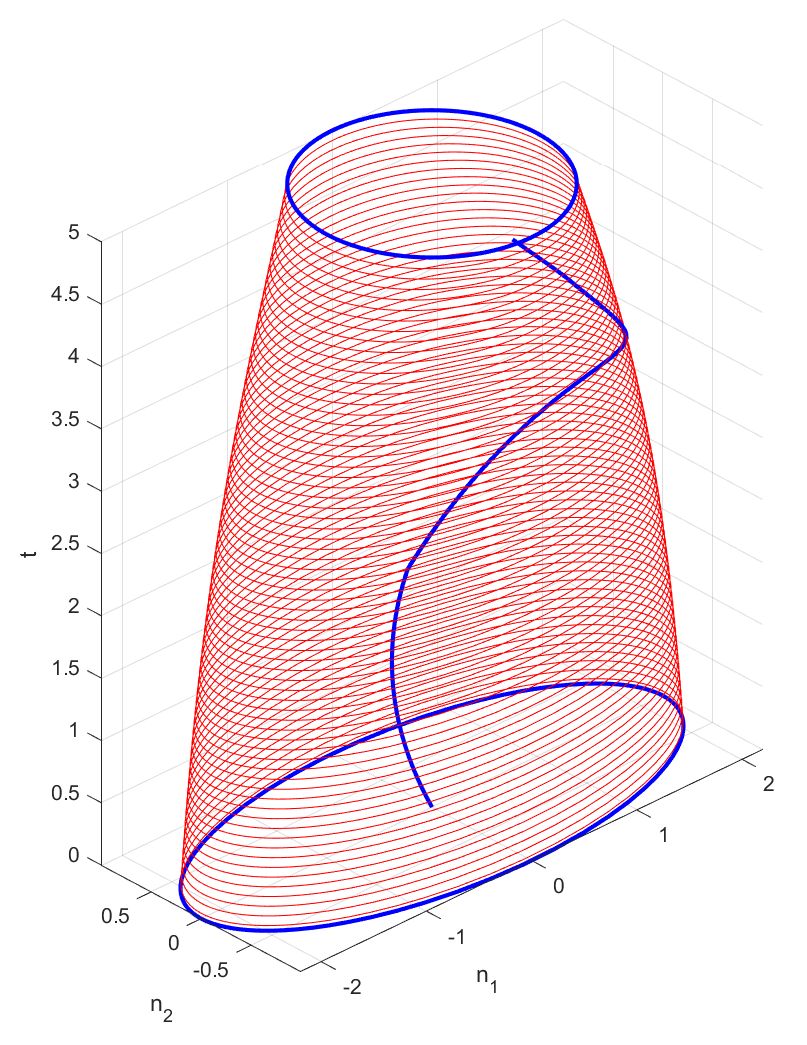
\includegraphics[width = 1 \textwidth]{evolution_first_example_cropped.pdf}
      \end{figure}
  \end{minipage}
  
\end{frame}

\begin{frame}{Пример 2}
  \begin{minipage}{0.45\textwidth}
  Изменим матрицы конфигурации ограничений на помеху и управление.
    \begin{gather*}
        P(t) = \begin{bmatrix}
            sin(3t) + 2 & 0 \\[0.3em]
            0 & sin(3t) + 2
        \end{bmatrix}, \\
        Q(t) = \begin{bmatrix}
            cos(3t) + 2 & 0 \\[0.3em]
            0 & cos(3t) + 2
        \end{bmatrix},
    \end{gather*}
    В этом случае ограничения на управление и помеху поочередно "доминируют" \ друг на другом, поэтому соответствующий альтернированный  интеграл с течением времени расширяется и сужается.
  \end{minipage} \hfill
  \begin{minipage}{0.5\textwidth}
      \begin{figure}
        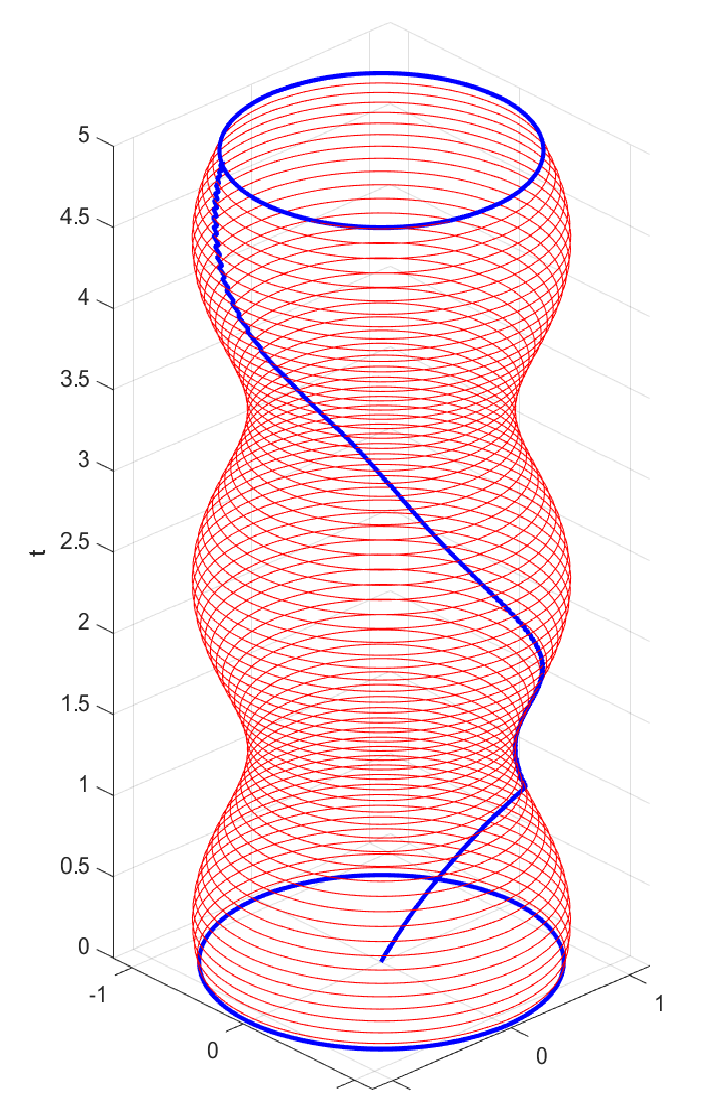
\includegraphics[width = 0.8 \textwidth]{evolution_with_touch_3_cropped.pdf}
      \end{figure}
  \end{minipage}
 
\end{frame}

\begin{frame}{Пример решения более общей задачи}
  \small
  Рассмотрим линейную систему с постоянными матрицами:
  \begin{equation*}
    \dot{x}(t) = Ax(t) + Bu(t) + Cv(t)
  \end{equation*}
  Где
  \footnotesize
  \begin{gather*}
    A = \begin{bmatrix}
        0 & 1 & 0 & 0 \\[0.3em]
        -1 & 0 & 0 & 0 \\[0.3em]
        0 & 0 & 0 & 1 \\[0.3em]
        0 & 0 & -4 & 0 
    \end{bmatrix},
    B = C = \begin{bmatrix}
        1 & 0 & 0 & 0 \\[0.3em]
        0 & 1 & 0 & 0 \\[0.3em]
        0 & 0 & 1 & 0 \\[0.3em]
        0 & 0 & 0 & 1 \\[0.3em]
    \end{bmatrix}, \\
    m = \begin{bmatrix}
        10 \\[0.3em]
        0 \\[0.3em]
        0 \\[0.3em]
        10
    \end{bmatrix},
    M = \begin{bmatrix}
        0.1 & 0 & 0 & 0 \\[0.3em]
        0 & 0.1 & 0 & 0 \\[0.3em]
        0 & 0 & 0.1 & 0 \\[0.3em]
        0 & 0 & 0 & 0.1
    \end{bmatrix},
    p(t) = \begin{bmatrix}
        0 \\[0.3em]
        0 \\[0.3em]
        0 \\[0.3em]
        0
    \end{bmatrix},
    P(t) = \begin{bmatrix}
        4 & 0 & 0 & 0 \\[0.3em]
        0 & 4 & 0 & 0 \\[0.3em]
        0 & 0 & 4 & 0 \\[0.3em]
        0 & 0 & 0 & 4
    \end{bmatrix}, \\
    q(t) = \begin{bmatrix}
        0 \\[0.3em]
        0 \\[0.3em]
        0 \\[0.3em]
        0
    \end{bmatrix},
    Q(t) = \begin{bmatrix}
        1 & 0 & 0 & 0 \\[0.3em]
        0 & 1 & 0 & 0 \\[0.3em]
        0 & 0 & 1 & 0 \\[0.3em]
        0 & 0 & 0 & 1
    \end{bmatrix},
    x_0 = \begin{bmatrix}
        3 \\[0.3em]
        -11 \\[0.3em]
        3 \\[0.3em]
        -10
    \end{bmatrix},
    v_1(t) = \begin{bmatrix}
        0 \\[0.3em]
        0 \\[0.3em]
        0 \\[0.3em]
        -1 \\[0.3em]
    \end{bmatrix},
    v_2(t) = \begin{bmatrix}
        0 \\[0.3em]
        0 \\[0.3em]
        0 \\[0.3em]
        1 \\[0.3em]
    \end{bmatrix}.
  \end{gather*}
\end{frame}

\begin{frame}{Иллюстрация траектории с коррекцией и целевого множества для первой помехи}

    \begin{figure}[ht]
    \centering
    \begin{subfigure}[b]{0.45\textwidth}
        \centering
        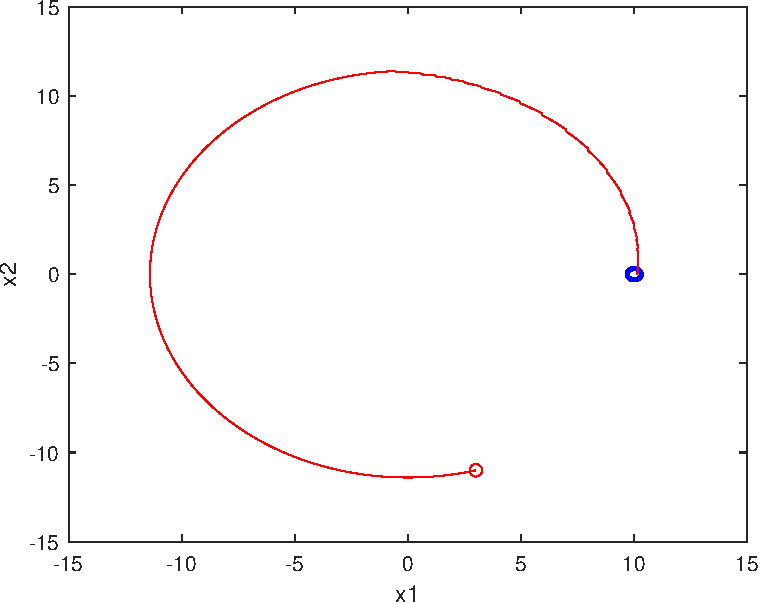
\includegraphics[width=\textwidth]{synthesis_8_first.pdf}
        \caption{Проекция на координаты первого осциллятора.}
        \label{subfig:synthesis_1_first}
    \end{subfigure}
    \hfill
    \begin{subfigure}[b]{0.45\textwidth}
        \centering
        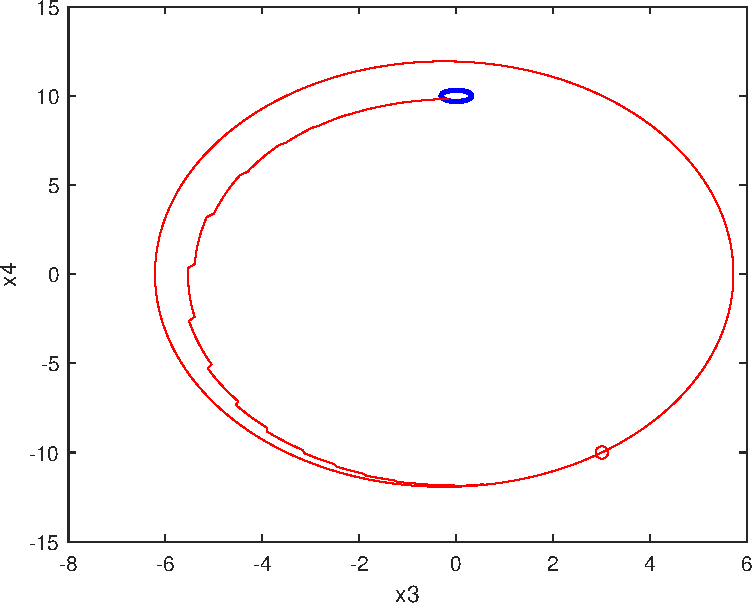
\includegraphics[width=\textwidth]{synthesis_8_second.pdf}
        \caption{Проекция на координаты второго осциллятора}
        \label{subfig:synthesis_1_second}
    \end{subfigure}
    \label{fig:synthesis_1}
    \end{figure}
    
\end{frame}
    
\begin{frame}{Иллюстрация траектории с коррекцией и целевого множества для второй помехи}
    \begin{figure}[ht]
    \centering
    \begin{subfigure}[b]{0.45\textwidth}
        \centering
        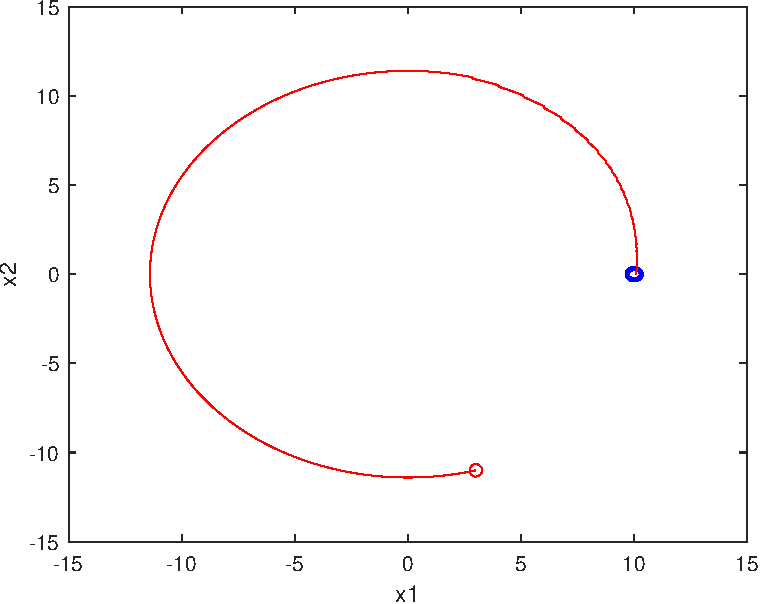
\includegraphics[width=\textwidth]{synthesis_9_first.pdf}
        \caption{Проекция на координаты первого осциллятора.}
        \label{subfig:synthesis_2_first}
    \end{subfigure}
    \hfill
    \begin{subfigure}[b]{0.45\textwidth}
        \centering
        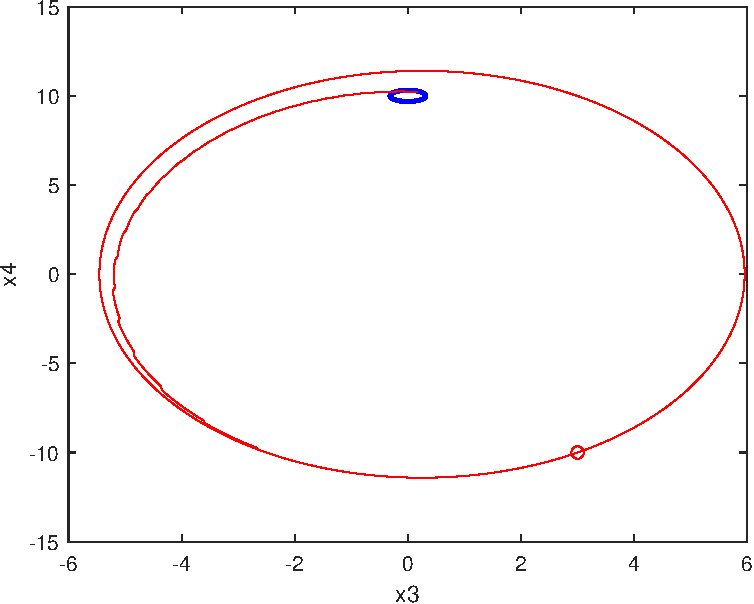
\includegraphics[width=\textwidth]{synthesis_9_second.pdf}
        \caption{Проекция на координаты второго осциллятора}
        \label{subfig:synthesis_2_second}
    \end{subfigure}
    \label{fig:synthesis_2}
    \end{figure}
    
\end{frame}

\begin{frame}{Детали численного метода}
\small
\begin{itemize}
    \item Функции \( x^*(t), X_-(t) \) для центра и матрицы конфигурации эллипсоидальной оценки ищутся на временной сетке с помощью метода Эйлера.
    \item На каждом шаге метода Эйлера ортогональная матрица \( H(t) \) ищется из сингулярного разложения векторов
    \begin{equation*}
        v(t) = (P(t))^{1/2} l, \quad w(t) = \frac{\langle l, P(t) l \rangle^{1/2}}{\langle l, X_-(t) l \rangle^{1/2}} (X_-(t))^{1/2} l
    \end{equation*}
    в виде
    \begin{equation*}
        H(t) = V_{w(t)} V_{v(t)}^T,
    \end{equation*}
    где матрицы \( V_{w(t)}, \ V_{v(t)} \) получаются из разложений:
    \begin{equation*}
    v(t) = V_{v(t)} \Sigma_{v(t)} u_{v(t)}, \quad w(t) = V_{w(t)} \Sigma_{w(t)} u_{w(t)}.
    \end{equation*}
    \item Значение лагранжевого множителя \( \lambda \) также ищется итерационно среди \( \lambda > 0 \) в силу свойств функции \( f(\lambda) \).
\end{itemize}
    
\end{frame}

\begin{frame}{Направления дальнейшей работы}
    \begin{itemize}
        \item Задачи с неопределенностью приводят к появлению геометрической разности в формулах для альтернированного интеграла и, соответственно, в эволюционных уравнениях для эллипсоидальных оценок. В связи с этим поиск параметров \( H(t), \pi(t) \) в дифференциальных уравнениях на матрицу конфигурации из условий касания, то есть равенства опорных функций для некоторых направлений, в приведенном выше виде невозможен. Таким образом, в алгоритм необходимо внедрять методы решающие эту проблему.
        \item Внедрение средств параллельного программирования для вычисления внутренних оценок.
        \item Изучение алгоритмов овыпукления функций для решения задач с неопределенностью.
        \item Решение конкретной прикладной задачи с помощью разобранной методики.
    \end{itemize}
\end{frame}

\begin{frame}{Список литературы}
    \small
    \begin{thebibliography}{0}
	
	\bibitem{ellips_calculus} Kurzhanki~A.\,B., \ Vâlyi~I.
	\emph{Ellipsoidal calculus for estimation and control}, Boston: Birkhäuser, 1996
	
	\bibitem{dyn_contr_traj_tubes}
	Kurzhanski~A.\,B., \ Varaiya~P. \emph{Dynamics and Control of Trajectory Tubes. Theory and Computation}, Springer, 2014

	\bibitem{reach_an_unc_sys} Kurzhanski~A.\,B., \ Varaiya~P. 
	\emph{Reachability Analysis for Uncertain Systems — the Ellipsoidal Technique}, Journal of Dynamics of Continuous, Discrete and Impulsive Systems, Ser. B., v.9, No 3, 2002, pp. 347–367.
    
	\bibitem{lin_dif_chasing} Понтрягин~Л.\,С.
	\emph{Линейные дифференциальные игры преследования}, Матем. сб., 1980, том 112(154), номер 3(7), 307-330
	
	\bibitem{el_toolbox_man} Kurzhanski~A.\,A., \ Gagarinov~P. 
	\emph{Ellipsoidal toolbox manual}, Release 2.0.1, 2014.
	
\end{thebibliography}
\end{frame}

\end{document}